% !TeX spellcheck = en_US
% !TeX encoding = UTF-8
% !LW recipe=latexmk (latexmkrc)
\documentclass{ifacconf}

% ------------------- debug cleveref and ifacconf -----------------------------
\newcounter{part}
\counterwithin*{section}{part}
%% ===================== packages ===========================================
\usepackage{fontspec}
\usepackage[utf8]{inputenc}
\usepackage{amsmath,amssymb,dutchcal,mathtools,siunitx,physics,etoolbox,minted}
\usepackage{booktabs,graphicx,xcolor,colortbl,natbib,tikz}
\usepackage[capitalize]{cleveref}
\usepackage[qtmarkupright]{glosmathtools}
%% =============== preamble ==================================================
%% ---------------- tikz -----------------------------------------------------
\usetikzlibrary{arrows,shapes.geometric}
%%generate seperate PDF for each tikz (compile with pdflatex -shell-escape) :
%\usetikzlibrary{external}
%\tikzexternalize[prefix=fig/]
%% ------------- glosmathtools -----------------------------------------------
\newignoredglossary{ignoredglos} % vectors are not printed in nomenclature
\loadglsentries{mpcPackageJulia_glos}
%% ----------------- amsmath -------------------------------------------------
\DeclareMathOperator{\diag}{diag}
%% ----------------- fontspec -------------------------------------
%\setmonofont{DejaVu Sans Mono}
%% ============================================================================

\setminted[julia]{%
    %linenos,
    %numbersep=3pt,
    %firstnumber=last,
    fontsize=\footnotesize,
    %frame=lines,
    %framesep=-5mm,
    bgcolor=gray!10,
}
\setminted[julia-repl]{%
    fontsize=\footnotesize,
    %frame=bottomline,
    %framesep=2mm,
    %framerule=10mm,
    %bgcolor=white
}

\newcommand*{\textttsmall}[1]{\texttt{\footnotesize #1}}

\begin{document}
\begin{frontmatter}

\title{ModelPredictiveControl.jl: advanced process control made easy in Julia}

\author[First]{Francis Gagnon} 
\author[First]{Alex Thivierge} 
\author[Second]{André Desbiens}

\address[First]{Jumine Inc., Quebec City, G1S 2K4, Canada}
\address[Second]{Process Observation and Optimization Laboratory (LOOP), Université Laval, Quebec City, G1V 0A6, Canada}

\begin{abstract} 
Sit commodo ipsum nulla eu excepteur sit ut minim voluptate et eu velit sint. Lorem et amet incididunt officia id. Nulla magna fugiat incididunt veniam sunt excepteur in esse nulla et aliquip non magna deserunt. 
\end{abstract}

\begin{keyword}
Model-based Control
\end{keyword}

\end{frontmatter}

% !TeX encoding = UTF-8
% !TeX spellcheck = en_US
\section{Introduction}

The process control community, both in the academic and industrial sectors, has largely relied on MATLAB toolboxes and commercial solutions for designing, simulating and implementing closed-loop systems \citep{optimMatlab}. The ecosystem developed by MathWorks\texttrademark\ is rich, mature, cohesive, and well documented, but their licensing policy can be unaffordable for smaller organizations. Moreover, because it is a proprietary software, the source code of many functions is not available. This is an issue for scientific research, where reproducibility and transparency is a key aspect. The dependency on a single vendor also raises concerns about the long-term support of third-party control software products. Lastly, like any interpreted languages e.g., Python, its performance can be suboptimal for computationally intensive tasks, especially for time-critical applications like real time optimization and model predictive control \citep{matlabPythonJulia, juliaML}. Code generation mitigates this issue, but it creates other problems like additional licensing fees, the difficulty to debug the generated code, and the restriction to a subset of the language.

Julia is relatively new programming language specialized for scientific and numerical computing. The just-ahead-of-time compiler can reach performance comparable to C and Fortran, while exhibiting a modern and expressive syntax like MATLAB and Python \citep{juliaPaper}. The built-in read-eval-print-loop (REPL) allows to interactively test code and inspect variables, mimicking the development workflow of an interpreted language. It also includes a package manager with a general registry, which makes it easy to share, install or update code. Moreover, the environment is free and open-source and it can be used for commercial purposes without any licensing fees. The ecosystem is still young, but a control toolbox (\texttt{ControlSystems.jl}), a system identification (\texttt{ControlSystemIdentification.jl}) and an optimization (\texttt{JuMP.jl}) packages are already available \citep{controlsystems, jump}. There is no free and open-source model predictive control (MPC) toolset available yet in the official registry of Julia, which is the gap this work fills.

This paper presents an MPC package for Julia. It aims to provide a simple, clear and modular framework to quickly design and test predictive controllers in Julia, while preserving the flexibility for advanced real-time optimization. For now, the package does particularly endeavor for original methodological scientific contributions or bleeding edge technologies like collocation methods or robust MPC, but rather to improve the accessibility to advanced process control, both for the academic and industrial community. With the exception of the petrochemical sector, many facilities still run their processes entirely in open-loop or with simple local controllers \citep{gapMPC}. Advanced process control can significantly reduce the waste in raw material and energy consumption. This is highly needed in the context of climate changes and the increasing scarcity of resources.

It focuses on modern MPCs that rely on a closed-loop state estimator for the feedback. The package currently implements the Luenberger observer and all the classical Kalman-type filters. It also incorporates an internal model control structure, as a more traditional approach. In addition, the analog of predictive control but for state estimation, the moving horizon estimator (MHE), is also available to solve constrained estimation problems. The user can also provide its own feedback strategy by defining a new state estimator subtype.

Linear plant models are automatically augmented with an adequate representation of the unmeasured disturbances based on observability (customizable). For the nonlinear case, the user chooses to add integrated white noise on the input or output for each channel. The \texttt{JuMP.jl} interface allows changing the solver quickly among  many open-source and commercial optimization software (local and global). As generic Julia functions can be differentiated using automatic differentiation , the gradient and Jacobian of the objective/constraint function for nonlinear MPCs are computed automatically with the machine precision. This also applies for the extended Kalman Filter. 

Additionally, by leveraging the multiple dispatch paradigm of Julia, nonlinear controllers based on linear models (e.g., economic MPC) evaluate the predictions with matrix algebra instead of a \texttt{for} loop, which is generally more efficient especially for the constraint handling. More precisely, the package functions dispatch on both the types of the controller and the plant model to select the most efficient implementation. Both soft and hard constraints on inputs, input increments, outputs, and terminal states are supported. The MHE state and noise estimates also support constraint relaxation.

The next section presents the structure and the main features of the package. The following one present two case studies to illustrate the syntax and benchmark the performances: a linear and a nonlinear controller design.
% !TeX encoding = UTF-8
% !TeX spellcheck = en_US

\section{Materials and Methods}

The functions of this package dispatch over three abstract types :
\begin{description}
    \item[SimModel] (2 subtypes) -- Discrete state-space models of the plant, including linear and nonlinear representations. Constructors automatically discretize 
    continuous-time linear systems. Instances of \texttt{SimModel} serves as a wrapper to construct \texttt{StateEstimator} and \texttt{PredictiveController} objects, and also as plant simulators to test the designs.
    \item[StateEstimator] (\replaced{7}{6} subtypes) -- Open loop and closed-loop state observers, both for deterministic and stochastic systems. They produce the full state feedback for the \texttt{PredictiveController}.
    \item[PredictiveController] (3 subtypes) -- Linear and nonlinear MPC are available. An explicit controller based on matrix algebra is also possible for linear models without constraint.
\end{description}

\subsection{Plant Models}

Plant models are defined by the abstract type \texttt{SimModel}. Operating points on the model inputs, outputs and measured disturbances are explicitly defined by the user. There are currently two concrete subtypes in the package, introduced in the following two sections.

\subsubsection{\textnormal{\texttt{LinModel}}}

Discrete linear state-space representations of the plant. Continuous-time models are discretized using zero-order hold for the manipulated inputs, and Tustin's approximation, for the measured disturbances (sampled continuous signals, usually). This leads to equations of the form:
\begin{subequations}
\begin{align}
    \mathbf{x}(k+1) &= \mathbf{A x}(k) + \mathbf{B_u u}(k) + \mathbf{B_d d}(k) \\
    \mathbf{y}(k)   &= \mathbf{C x}(k) + \mathbf{D_d d}(k)
\end{align}
\end{subequations}
in which the vectors $\mathbf{u}$, $\mathbf{d}$, $\mathbf{x}$ and $\mathbf{y}$ are the manipulated input, measured disturbance, state and output of the model, respectively. Objects are constructed with \texttt{ss} or \texttt{tf} functions from \texttt{ControlSystems.jl}, or by providing the fives state-space matrices directly.

\subsubsection{\textnormal{\texttt{NonLinModel}}}

Discrete nonlinear state-space representations of the plant. \replaced[comment={now supported}]{A built-in 4th order Runge-Kutta solver with optional supersampling discretizes continuous-time dynamics by default, leading to the following system of equations:}{Continuous-time models are not supported yet but manually calling a differential equation solver can mitigate this (see Section 3.2 example). The user provides the following two functions:}. 
\begin{subequations}
\begin{align}
    \mathbf{x}(k+1) &= \mathbf{f}\big(\mathbf{x}(k), \mathbf{u}(k), \mathbf{d}(k)\big) \\
    \mathbf{y}(k)   &= \mathbf{h}\big( \mathbf{x}(k), \mathbf{d}(k) \big)
\end{align}
\end{subequations}
It is worth mentioning that the state update $\mathbf{f}$ and output $\mathbf{h}$ functions must be in pure Julia to design nonlinear MPCs from them, since the implementation rely on automatic differentiation.

\subsection{State Estimators}

The estimators of the package focus on control applications, that is, relying on the estimates to compute a full state feedback. They all incorporate some kind of integral action by default if feasible, since it is generally desired to eliminate the steady-state error with closed-loop control (offset-free tracking). \cref{sec:case_studies} gives details on that matter.

\replaced{At the time of writing, they are all}{They are also} implemented in the predictor form (a.k.a. \replaced{delayed estimator}{observer form}), that is, they all estimates at each discrete time $k$ the states of the next period $\mathbf{\hat{x}}_k(k+1)$, also denoted $\mathbf{\hat{x}}(k+1|k)$. \replaced{This approach induces a one-sample time delay in the feedback and its accuracy is slightly lower than the current form that estimates $\mathbf{\hat{x}}_k(k)$.}{In comparison to the filter form that estimates $\mathbf{\hat{x}}_k(k)$,  is sometimes slightly more accurate.} The predictor form \replaced{is however}{comes in} handy for control applications since the estimations come after the controller computations, without introducing any additional delays. This is especially true if the observer computations are expensive \added{e.g.: the MHE}. \added[comment={will work on that while co-authors revise the manuscript}]{The support for current estimators will be added soon after this submission to let the user decide.}

There \replaced{are seven}{is six} \texttt{StateEstimator} concrete types available at the time of writing, all supporting measured $\mathbf{y^m}$ and unmeasured $\mathbf{y^u}$ model outputs. \deleted{The moving horizon estimator will be added soon after this publication.}The following list presents them.

\subsubsection{\textnormal{\texttt{SteadyKalmanFilter}}}
Steady-state Kalman filter, a.k.a. asymptotic form. The solution to the algebraic Riccati equation pre-compute the Kalman gain \citep{simon}. This is the default state estimator for controllers based on \texttt{LinModel} objects.

\subsubsection{\textnormal{\texttt{KalmanFilter}}}
Time-varying version of the Kalman filter. It can evaluate the estimation error covariance in real time or be applied in situations where there is no solution to the algebraic Riccati equation.

\subsubsection{\textnormal{\texttt{Luenberger}}}
Deterministic state observer based on closed-loop eigenvalue placement. It pre-computes the observer gain with \texttt{place} function from \texttt{ControlSystems.jl}, that implements the method of \citet{placePoles}.

\subsubsection{\textnormal{\texttt{UnscentedKalmanFilter}}}
Kalman filter for nonlinear systems relying on the generalized unscented transform \citep{simon}. It propagates the mean and covariance of the noise by approximating the state probability distribution instead of linearizing the model like the \texttt{ExtendedKalmanFilter}. This is the default state estimator for controllers based on \texttt{NonLinModel} objects.

\subsubsection{\textnormal{\texttt{ExtendedKalmanFilter}}}
Extended form of the time-varying Kalman filter. The Jacobians of the nonlinear state-space functions approximate the propagation of the noise. These matrices are automatically computed by forward mode automatic differentiation.

\subsubsection{\textnormal{\texttt{MovingHorizonEstimator}}}
\added{%
Also known as receding horizon estimation. It minimizes at each discrete time $k$ the following cost function over an estimation window of $N_k = \min(k+1, H_e)$ steps, where $H_e$ is the estimation horizon:
\begin{equation}\label{eq:J_MHE}
    J_{\mathit{MHE}} = \bar{\mathbf{x}}^\intercal \bar{\mathbf{P}}^{-1} \bar{\mathbf{x}} 
    + \mathbf{\hat{W}}^\intercal \mathbf{\hat{Q}}_{N_k}^{-1} \mathbf{\hat{W}}  
    + \mathbf{\hat{V}}^\intercal \mathbf{\hat{R}}_{N_k}^{-1} \mathbf{\hat{V}}
    + C \epsilon^2
\end{equation}
The state estimate at arrival $\mathbf{\hat{x}}_k(k-N_k+1)$, the process noise estimates over the window $\mathbf{\hat{W}}$ and the slack variable $\epsilon$ for constraint relaxation are the decision variables. The process and disturbance models compute the sensor noise estimates $\mathbf{\hat{V}}$. The estimation error $\bar{\mathbf{x}} = \mathbf{\hat{x}}_{k-N_k}(k-N_k+1) - \mathbf{\hat{x}}_{k}(k-N_k+1)$ and its covariance $\bar{\mathbf{P}} = \mathbf{\hat{P}}_{k-N_k}(k-N_k+1)$
evaluate the arrival costs. The block diagonal matrices $\mathbf{\hat{Q}}_{N_k}$ and $\mathbf{\hat{R}}_{N_k}$ comprise the noise covariances.
}%

\added{%
This approach allows incorporating additional physical information on the process an its disturbances, in the form of constraints on the state and noise estimates:
\begin{alignat}{3}
    \mathbf{\hat{X}_{min} - C_{\hat{x}_{min}}} \epsilon &\le \mathbf{\hat{X}} &&\le \mathbf{\hat{X}_{max} + C_{\hat{x}_{max}}} \epsilon \\
    \mathbf{\hat{W}_{min} - C_{\hat{w}_{min}}} \epsilon &\le \mathbf{\hat{W}} &&\le \mathbf{\hat{W}_{max} + C_{\hat{w}_{max}}} \epsilon \\
    \mathbf{\hat{V}_{min} - C_{\hat{v}_{min}}} \epsilon &\le \mathbf{\hat{V}} &&\le \mathbf{\hat{V}_{max} + C_{\hat{v}_{max}}} \epsilon
\end{alignat}
and also $\epsilon \ge 0$. The $\mathbf{\hat{X}}$ vectors gather the state estimates over the window. The $\mathbf{C}$ vectors are non-negative values that specify the softness of the associated bound, and $C$ globally weights the slack $\epsilon$ (equal concern for relaxation). The problem \eqref{eq:J_MHE} is treated as a quadratic program for \texttt{LinModel}, and a nonlinear optimization, for \texttt{NonLinModel}.
}%

\subsubsection{\textnormal{\texttt{InternalModel}}}
Allows the design of predictive controllers based on an internal model structure. It is based on the general approach of \citet{globPC}. The stochastic model of the unmeasured disturbances defaults to integrating white noise for each measured output (customizable). This is the equivalent of assuming that the disturbances are constant over the prediction horizon, similarly to dynamic matrix control (DMC). It supports asymptotically stable \texttt{LinModel} or \texttt{NonLinModel}.

\subsection{Predictive Controllers}

The prediction methodology applied throughout the package is mainly based on the textbook of \citet{mpcMac}. The three \texttt{PredictiveController} types are presented in the following sections.

\subsubsection{\textnormal{\texttt{LinMPC}}}
Linear model predictive controller with constraints. It minimizes the following objective function at each discrete time $k$:
\begin{multline}\label{eq:J_MPC}
J_{\mathit{MPC}} = 
    \mathbf{\big(\hat{R}_y - \hat{Y}\big)}^\intercal \mathbf{M}_{H_p} \mathbf{\big(\hat{R}_y - \hat{Y}\big)}   
    + \mathbf{\big(ΔU\big)}^\intercal \mathbf{N}_{H_c} \mathbf{\big(ΔU\big)} \\
    + \mathbf{\big(\hat{R}_u - U\big)}^\intercal \mathbf{L}_{H_p} \mathbf{\big(\hat{R}_u - U\big)} 
    + C \epsilon^2
\end{multline}
with the decision variables $\mathbf{ΔU}$ and $\epsilon$, the inputs increments over the control horizon $H_c$ and the slack variable\deleted{ for relaxation}, respectively. The vectors $\mathbf{\hat{Y}}$ and $\mathbf{\hat{R}_y}$ encompass the predictions of the outputs and their setpoints over the horizon $H_p$, respectively. The variables $\mathbf{U}$ and $\mathbf{\hat{R}_u}$ are similar but for the input setpoints. The matrices $\mathbf{M}_{H_p}$, $\mathbf{N}_{H_c}$ and $\mathbf{L}_{H_p}$ are \replaced[comment={no longer restricted to diagonal}]{Hermitian}{diagonal} weights \deleted[comment={move above in the new MHE section}]{, and $C$ is a scalar weight}. 

The problem is subject to the following constraints:
\begin{alignat}{3}
    \mathbf{U_{min}  - C_{u_{min}}}  \epsilon &\le \mathbf{U}  &&\le \mathbf{U_{max}  + C_{u_{max}}}  \epsilon \\
    \mathbf{ΔU_{min} - C_{Δu_{min}}} \epsilon &\le \mathbf{ΔU} &&\le \mathbf{ΔU_{max} + C_{Δu_{max}}} \epsilon \\
    \mathbf{Y_{min}  - C_{y_{min}}}  \epsilon &\le \mathbf{\hat{Y}} &&\le \mathbf{Y_{max}  + C_{y_{max}}}  \epsilon
\end{alignat}
and also $\epsilon \ge 0$. \deleted[comment={moved above in the new MHE section}]{The $\mathbf{C}$ vectors are non-negative values that specify the softness of the associated bound (equal concern for relaxation).} Box constraints on the terminal states are also possible: $\mathbf{\hat{x}_{min}} {-} \mathbf{c_{\hat{x}_{min}}}\epsilon \le \mathbf{\hat{x}}_{k-1}(k{+}H_p) \le \mathbf{\hat{x}_{max}} + \mathbf{c_{\hat{x}_{max}}}\epsilon$. Note that changing the bounds at runtime and time-varying constraints over the horizons are supported.

The default optimizer is \texttt{OSQP.jl} that efficiently handles sparse problems \citep{osqp}, but the \texttt{JuMP.jl} interface allows switching among many quadratic solvers. For example, the dual active-set method of \citet{daqp} is sometimes faster on small and dense matrices. Testing this solver only takes one line of code.

\subsubsection{\textnormal{\texttt{ExplicitMPC}}}
Linear model predictive controller without constraints, see \texttt{LinMPC} for the cost function. The computational costs are extremely low (\added{the analytical solution of the quadratic problem leads to a single} array division), therefore suitable for applications that require small sample times. \added{It produces a control law similar to a finite-horizon linear-quadratic regulator (LQR), but with the control horizon $H_c$, the move suppression $\mathbf{N}_{H_c}$ and the input setpoint tracking $\mathbf{L}_{H_p}$ weights available as additional tuning parameters.}

\subsubsection{\textnormal{\texttt{NonLinMPC}}}
Nonlinear model predictive controller with constraints. The objective function includes an additional term for economic MPC:
\begin{equation}
J_{\mathit{NMPC}} = J_{\mathit{MPC}} 
    + E J_E\big(\mathbf{U}_E, \mathbf{\hat{Y}}_E, \mathbf{\hat{D}}_E\big)
\end{equation}
with $J_{\mathit{MPC}}$ from \eqref{eq:J_MPC}. The user provides a custom function $J_E$ that returns the economic costs for a given set of inputs $\mathbf{U}_E$, outputs $\mathbf{\hat{Y}}_E$ and measured disturbances $\mathbf{\hat{D}}_E$:
\begin{equation}
\mathbf{U}_E = 
\begin{bmatrix}
    \mathbf{U} \\ \mathbf{u}(k+H_p-1)
\end{bmatrix}\!,\,
\mathbf{\hat{Y}}_E = 
\begin{bmatrix}
    \mathbf{\hat{y}}(k) \\ \mathbf{\hat{Y}}
\end{bmatrix}\!,\, 
\mathbf{\hat{D}}_E = 
\begin{bmatrix}
    \mathbf{d}(k) \\ \mathbf{\hat{D}}
\end{bmatrix} 
\end{equation} 
The constraint parameters are identical to \texttt{LinMPC}. The default optimizer is \texttt{Ipopt.jl}, an open-source interior point method developed by \citet{ipopt}.

% !TeX encoding = UTF-8
% !TeX spellcheck = en_US
\section{Case studies}

\subsection{Continously Stirred Tank Reactor}

\subsubsection{Linear Model}

The example considers a continuously stirred tank reactor with a hot and cold water intakes. The linear model, with the manipulated inputs $\mathbf{u}=\begin{smallmatrix}[
u_c & u_h]'\end{smallmatrix}$ and the liquid level and tempertaure as measured outputs $\mathbf{y}=\begin{smallmatrix}[y_L & y_T]'\end{smallmatrix}$ is constructed with:

\begin{minted}{julia}
using ModelPredictiveControl, ControlSystemsBase
sys = [ tf(1.90, [18, 1]) tf(1.90, [18, 1]);
        tf(-0.74,[8, 1])  tf(0.74, [8, 1]) ]
Ts = 2.0; uop = [20, 20]; yop = [50, 30]
model = setop!(LinModel(sys, Ts); uop, yop)
\end{minted}
\vspace{-26pt}
\begin{minted}{julia-repl}
Discrete-time linear model with a sample time 
Ts = 2.0 s and:
 2 manipulated inputs u
 2 states x
 2 outputs y
 0 measured disturbances d
\end{minted}

The figure 1 depicts the instrumentation installed on the plant. The \texttt{model} object will be used for two purposes : to construct our controller, and as a plant simulator to test the design.

\subsubsection{Linear Model Predictive Controller}

The objective is to control both the water temperature and level while constraining the level above 45:

\begin{minted}{julia}
nint_u = [1, 1]; ymin = [45, -Inf]
mpc = setconstraint!(LinMPC(model; nint_u); ymin)
\end{minted}
\vspace{-25pt}
\begin{minted}{julia-repl}
LinMPC controller with a sample time Ts = 2.0 s,
OSQP optimizer, SteadyKalmanFilter estimator and:
 15 prediction steps Hp
  2 control steps Hc
  2 manipulated inputs u (2 integrating states)
  4 states x̂
  2 measured outputs ym (0 integrating states)
  0 unmeasured outputs yu
  0 measured disturbances d
\end{minted}

By default, \texttt{LinMPC} controllers use \texttt{OSQP.jl} to solve the problem, soft constraints on output predictions $\mathbf{\hat y}$ to ensure feasibility, and a SteadyKalmanFilter to estimate the plant states\footnote{We could have use an InternalModel structure, to avoid state observer, with \texttt{mpc = LinMPC(InternalModel(model), Hp=15, Hc=2, Mwt=[1, 1], Nwt=[0.1, 0.1])}. It was tested on the example of this page and it gives similar results.}. An attentive reader will also notice that the Kalman filter estimates two additional states compared to the plant model. These are the integrating states for the unmeasured plant disturbances, added at the model inputs here.  

Before closing the loop, 

we initialize the estimates with the actual plant inputs and measurements to ensure a bumpless transfer. Since model simulates our plant here, its output will initialize the states. \texttt{LinModel} objects are callable for this purpose. 

We can then close the loop and test \texttt{mpc} performance on the simulator by imposing step changes on output setpoints $\mathbf{r_y}$ and on a load disturbance $u_l$:

\begin{minted}{julia}
function test_mpc(mpc, plant)
    plant.x[:] .= 0; y = plant() # or evaloutput(plant)
    initstate!(mpc, plant.uop, y)
    N = 75; ry = [50, 30]; ul = 0
    U_data, Y_data = zeros(plant.nu,N), zeros(plant.ny,N)
    Ry_data = zeros(plant.ny,N)
    for i = 1:N
        i == 26 && (ry = [48, 35])
        i == 51 && (ul = -10)
        y = plant() 
        u = mpc(ry) # or moveinput!(mpc, ry)
        U_data[:,i], Y_data[:,i], Ry_data[:,i] = u, y, ry
        updatestate!(mpc, u, y) # update mpc estimate
        updatestate!(plant, u+[0,ul])
    end
    return U_data, Y_data, Ry_data
end
U_data, Y_data, Ry_data = test_mpc(mpc, model)
\end{minted}

Updating the internal states of \texttt{mpc} prepares the object for the \emph{next} time step. That is why the call is done at the end of the \texttt{for} loop. The same logic applies for \texttt{model}. Lastly, we plot the closed-loop test with \texttt{Plots.jl}:

\begin{minted}{julia}
res = SimResult(mpc, U_data, Y_data; Ry_data)
using Plots; plot(res)
\end{minted}

\begin{figure}
    \centering
    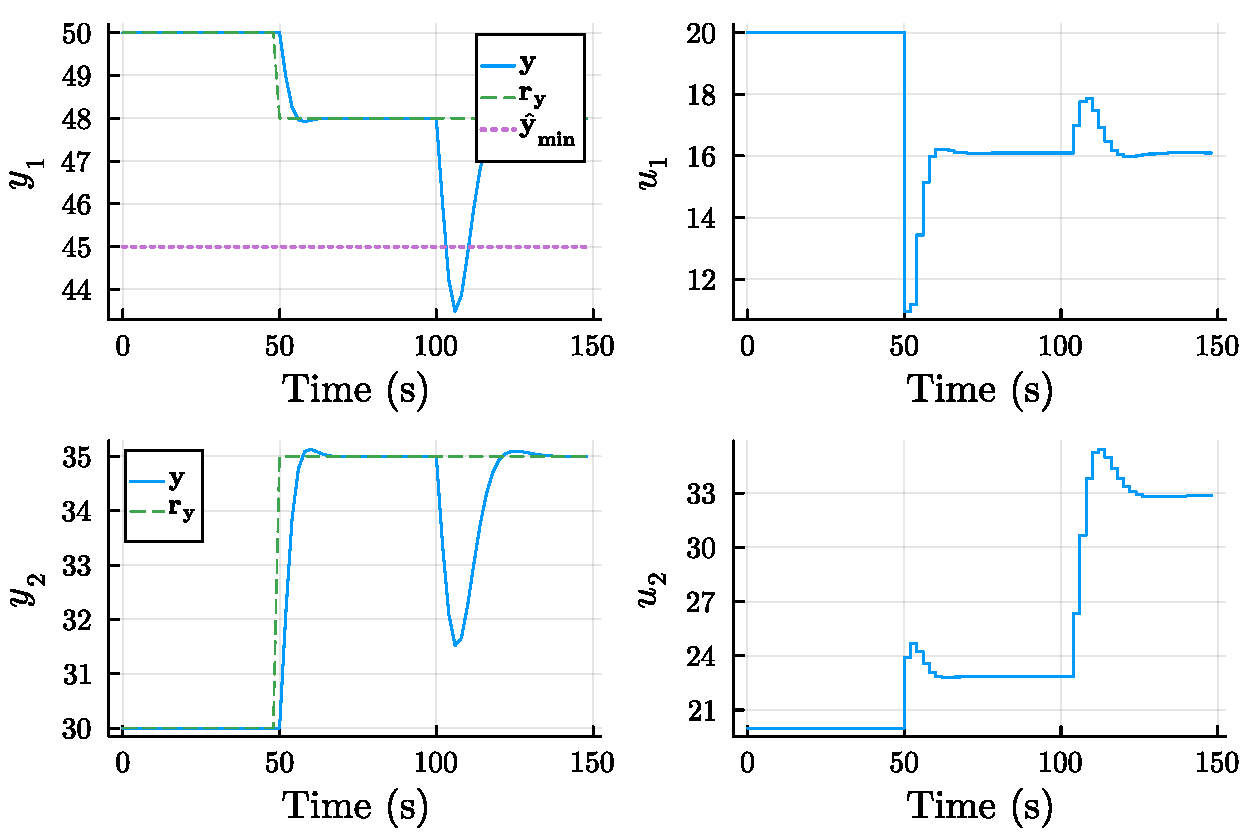
\includegraphics[width=\columnwidth]{fig/plot1_LinMPC.pdf}
    \caption{CSTR closed-loop simulation}
    \label{fig:plot1_LinMPC}
\end{figure}

\cref{fig:plot1_LinMPC} shows that the controller violates the constraints around 110 s because of the disturbance. Adding feedforward compensation can improve the performance.

\subsubsection{Feedforward Compensation}

Suppose that the load disturbance $u_l$ of the last section is in fact caused by a separate hot water pipe that discharges into the tank. Measuring this flow rate allows us to incorporate feedforward compensation:

\begin{minted}{julia}
model_d = LinModel([sys sys[1:2, 2]], Ts; i_d=[3])
model_d = setop!(model_d; uop, yop, dop=[20])
\end{minted}

The simulation needs an MPC based on \texttt{model\_ff} and a new test function that employs the measured disturbance:

\begin{minted}{julia}
mpc = setconstraint!(LinMPC(model_d; nint_u); ymin)
function test_mpc_ff(mpc, plant)
    plant.x[:] .= 0; y = plant(); d = [20]
    initstate!(mpc, plant.uop, y, d)
    N = 75; ry = [50, 30]; ul = 0
    U_data, Y_data = zeros(plant.nu,N), zeros(plant.ny,N)
    Ry_data = zeros(plant.ny,N)
    for i = 1:N
        i == 26 && (ry = [48, 35])
        i == 51 && (ul = -10)
        y = plant(); d = [20+ul]
        u = mpc(ry, d)
        U_data[:,i], Y_data[:,i], Ry_data[:,i] = u, y, ry
        updatestate!(mpc, u, y, d) 
        updatestate!(plant, u+[0,ul])
    end
    return U_data, Y_data, Ry_data
end
U_data, Y_data, Ry_data = test_mpc_ff(mpc, model)
plot(SimResult(mpc, U_data, Y_data; Ry_data))
\end{minted}

\cref{fig:plot2_LinMPC} shows that the compensation handles the disturbance without violating the constraint.

\begin{figure}
    \centering
    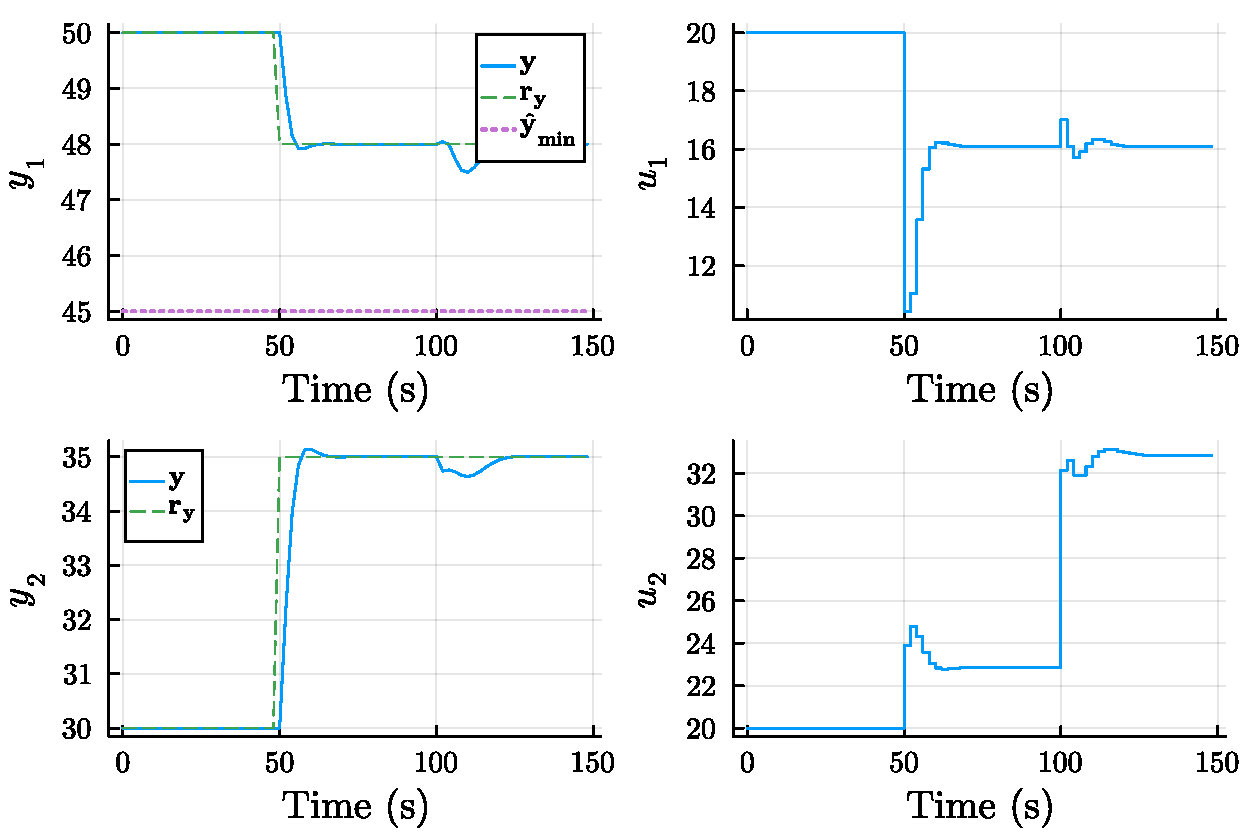
\includegraphics[width=\columnwidth]{fig/plot2_LinMPC.pdf}
    \caption{CSTR closed-loop simulation with feedforward}
    \label{fig:plot2_LinMPC}
\end{figure}

\subsection{Inverted Pendulum}



\section{Results and Discussion}
\label{sec.results_simple}

Laboris exercitation sunt adipisicing laboris nulla ad occaecat irure magna voluptate. Veniam eu labore Lorem anim nostrud minim Lorem fugiat nulla. Non anim veniam laborum deserunt adipisicing cillum aliquip deserunt pariatur consectetur consequat irure. Dolor aute incididunt quis magna. Dolor nostrud exercitation duis sunt nulla adipisicing enim laborum ex ut esse ad. Incididunt exercitation velit ea elit ut laboris eu amet.

Minim magna culpa ipsum do proident cillum sit. Officia ad et consequat do magna nostrud irure nostrud. Ipsum sunt adipisicing Lorem sunt tempor ex veniam consequat veniam ipsum. Aliquip voluptate labore mollit duis id mollit nulla id ipsum. Velit esse nisi qui pariatur ad nostrud.

Aute minim anim culpa minim aliquip sint laboris sunt. Ea ex tempor irure officia laborum est aliquip nostrud quis do. Lorem cupidatat mollit do officia aute in est cillum cillum consectetur laborum pariatur. Id tempor minim eiusmod ex laboris. Aute aliquip cupidatat nostrud aute dolor mollit ex commodo do excepteur dolor irure. Ut veniam amet id excepteur excepteur velit laboris aliqua sit occaecat irure dolor labore.

Proident ad minim magna minim excepteur reprehenderit elit id ipsum amet velit sunt aute aute. Consectetur excepteur velit quis aliqua sint laborum veniam minim proident. Veniam proident laboris aute deserunt do do amet qui pariatur occaecat cillum. Minim magna in et laborum ipsum deserunt pariatur cupidatat ipsum veniam aliqua elit. Aliqua id proident fugiat nisi esse eu nulla sint qui reprehenderit aliqua sunt. Cillum duis anim sit velit dolore.

\begin{table}[tb]
	\caption{Simplified model parameters for batch fluidized bed drying}
	\label{tab.simple_params}
	\centering
	% !TeX spellcheck = en_US

\begin{tabular}{l l l l}
	
\toprule %=======================================================================

parameter 			& value 	   		& \shortstack[l]{standard\\deviation} & units  \\

\midrule %-----------------------------------------------------------------
					
\glsub{chi}{0}    	& \num{0.15e-2}		& -- 					& --		\\

%--------------------------------------------------------------------------

\rowcolor{blue!10}
\gls{a1}			& \num{9.26e-5}		& \num{0.04e-5}		%
										& \si{\per\meter\cubed} \\
\rowcolor{blue!10}
\gls{b1}			& \num{4.54e-2}		& \num{0.05e-2}		%
										& \si{\degreeCelsius\per\meter\cubed} \\
\rowcolor{blue!10}					
\gls{b2}			& \num{2.56e-05}	& \num{0.02e-05}	%
										& \si{\per\meter\cubed}	 \\

%--------------------------------------------------------------------------

\rowcolor{blue!10}
\gls{nu}			& \num{3.48}		&  \num{0.12}		& -- \\		
\rowcolor{blue!10}
\glsub{chi}{pc}		& \num{2.33e-2}	 	&  \num{0.06e-2}	& -- \\
				
%-------------------------------------------------------------------------

\gls{alpha}   	   	& \num{4.90e-3} 	& --			& --  \\
\gls{beta}			& \num{5.70e-2}		& -- 			& \si{\per\degreeCelsius}\\

%----------------------------------------------------------------------------

\gls{tau}			& \num{86.7}		&--				& \si{\second}  \\

\bottomrule %====================================================================
	
\end{tabular}

\end{table}

Occaecat Lorem commodo in minim consectetur voluptate nostrud enim tempor incididunt laborum occaecat. Aliqua non et nulla voluptate amet sunt. Laboris nisi consequat cupidatat est consequat deserunt ipsum.

% !TeX encoding = UTF-8
% !TeX spellcheck = en_US
\section{Conclusion}

This paper introduced the \texttt{ModelPredictiveControl.jl} package, a free and open-source package for advanced process control in Julia. It relies on \texttt{ControlSystems.jl} and \texttt{JuMP.jl}, two powerful frameworks for computer-aided control system design and mathematical optimization, respectively. The new state estimator and predictive controller types are designed to be easy to use, clear and modular. The main features of the package were described and illustrated with two case studies. A benchmark comparison with the equivalent MATLAB toolbox exposes its computational efficiency, without any code generation, and thus avoiding the two-language problem. The package is still under active development and contributions are welcome. Short-term developments will focus on implementing estimators in the current form to eliminate the one-sample time delay when possible. Recent developments on abstraction interfaces to automatic differentiation libraries could be also integrated to facilitate the testing of other approaches like reverse- or mixed-mode.

\begin{ack}
Culpa in deserunt proident tempor non. Duis et esse pariatur esse qui duis exercitation ullamco aliquip. Dolore ipsum sint consequat enim laborum duis anim cupidatat.
\end{ack}

\bibliography{mpcPackageJulia_bibfile}


\end{document}